\section{Discovering Routing Proxies and DRAs}
\label{sec-proxy-algorithms}
From Section~\ref{subsec-proxy-properties}, it is easy to see that the remaining challenge is to discover \dras and their maximal proxies on large graphs.
In this section, we first present a notion of  \bcsketch graphs, based on which we then propose a linear-time algorithm  for computing \dras and their maximal proxies. This makes our solution a light weight approach to reducing graph sizes and to  speeding-up shortest  path and distance queries on large graphs.



The main result here is stated as follows.

\begin{theorem}
\label{thm-compute-dras} Finding all \dras, each associated with one maximal proxy, in a graph can be done in linear time.
\end{theorem}


We shall prove this by providing a linear time algorithm that computes \dras and maximal proxies.


\stitle{1. Connections with cut-nodes}. We first show that there are close connections between proxies and cut-nodes.



\begin{prop}
\label{prop-proxy-cut} Any proxy in a \cc $H(V_s, E_s)$ of graph $G(V$, $E)$ with $|V_s|>c\cdot\lfloor\sqrt{|V|}\rfloor$ must be a cut-node of graph $G$.
\end{prop}



\begin{prop}
\label{prop-large-bcc} Any node in a \bc with size larger than $c\cdot\lfloor\sqrt{|V|}\rfloor$ of graph $G(V$, $E)$ is a trivial proxy.
\end{prop}


This motivates us to identify (non-trivial maximal) proxies by utilizing the cut-nodes and \bccs, which will be seen immediately.
Further, as we are interested in non-trivial proxies only, those large \bccs could be simply ignored without any side effects.

%%%%%%%%%%%%%%%%%%%%%%%%%%%%%%%%%%%%%%%%%%%%%%%%%%
%%%%%%%%%%%%%%%%%%%%%%%%%%%%%%%%%%%%%%%%%%%%%%%%%%
\begin{figure}[tb!]
%\vspace{2ex}
\begin{center}
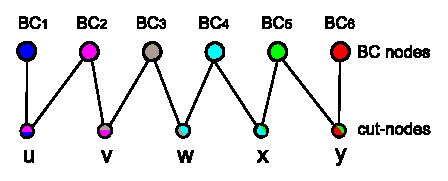
\includegraphics[scale=0.9]{./sketch-graphs.eps}
\end{center}
\vspace{-2ex}
\caption{\bcsketch graph $\mathbb{G}_1$ of graph $G_1$}
\label{fig-sketch-graph}\vspace{-3ex}
\end{figure}
%%%%%%%%%%%%%%%%%%%%%%%%%%%%%%%%%%%%%%%%%%%%%%%%%%

\stitle{2. \bcsketch graphs}. We then present \bcsketch graphs, which are defined in terms of cut-nodes and \bccs, and are a key notion employed by our algorithm.

A \bcsketch graph $\mathbb{G(V, E}, \omega)$ of a graph $G(V, E)$ is a bipartite graph, in which (1) $\mathbb{V}$ = $\mathbb{V}_{c}\cup \mathbb{V}_{bc}$
such that $\mathbb{V}_{c}$ is the set of cut-nodes in $G$, and $\mathbb{V}_{bc}$ is the set of \bccs in $G$;
(2) for each cut-node $v\in \mathbb{V}_{c}$ and each \bc $y_{b}\in \mathbb{V}_{bc}$, there exists an edge $(v, y_b)\in \mathbb{E}$ iff $v$ is a cut-node of \bc $y_b$;
and (3) $\omega$ is a weight function such that for each node $y_b\in \mathbb{V}_{bc}$, $\omega(y_b)$ is the number of nodes of $G$ in \bc $y_b$.




\vspace{-0.5ex}
\begin{example}
\label{exm-sketch-graph} Consider graph $G_1$ in Fig.~\ref{fig-cut-nodes}(1), and the corresponding \bccs of $G_1$ in Fig.~\ref{fig-cut-nodes}(2).



The \bcsketch graph $\mathbb{G}_1(\mathbb{V, E}, \omega)$ of graph $G_1$ is shown in Fig.~\ref{fig-sketch-graph},
in which $\omega(BC_1)$ = 4, $\omega(BC_2)$ = $\omega(BC_3)$ = $\omega(BC_4)$ = $\omega(BC_6)$ = 2, and $\omega(BC_5)$ = 5.
\end{example}

One may already notice that there are no cycles in the \bcsketch graph $\mathbb{G}_3$ in Fig.~\ref{fig-sketch-graph}. This is not a coincidence, as shown below.

\begin{prop}
\label{pro-sketch-graph} \bcsketch graphs have no cycles, which implies that they are simply trees.
\end{prop}



Proposition~\ref{pro-sketch-graph} indicates that the good properties of trees can be employed for computing \dras and maximal proxies.


\stitle{3. Algorithms}.
We are now ready to present algorithm \compDRAs shown in Fig.~\ref{alg-compute-proxies}, which takes as input graph $G$ and constant $c$, and outputs the \dras of $G$, each associated with a maximal proxy.

%%%%%%%%%%%%%%%%%%%%%Baseline Algorithm
\begin{figure}[tb!]
%\vspace{1ex}
\begin{center}
{\small
\begin{minipage}{3.2in}
\myhrule \vspace{-2ex}
\mat{0ex}{
{\bf Algorithm}~\compDRAs\\
\sstab {\sl Input:\/} \= Graph $G(V, E)$ and constant $c$.\\
{\sl Output:\/} \= The \dras with their maximal proxies. \\

\sstab\bcc\ \= Find all cut-nodes $\mathbb{V}_c$ and \bc nodes $\mathbb{V}_{bc}$ of $G$; \\
\icc\> Build the \bcsketch graph $\mathbb{G(V, E}, \omega)$ with  $\mathbb{V}$ = $\mathbb{V}_c\cup \mathbb{V}_{bc}$;\\
\icc\> Identify and return \dras with their maximal proxies of $G$.
}

\vspace{-2ex}
\mat{0ex}{
{\bf Procedure}~$\kw{extractDRAs}$\\
\sstab {\sl Input:\/} \= \bcsketch graph $\mathbb{G(V, E}, \omega)$ of graph $G$ and constant $c$.\\
{\sl Output:\/} The \dras and their maximal proxies of $G$.\\
\bcc \hspace{1.8ex}\= \Let $F$ be the set of cut-nodes with single non-leaf  \\
\>neighbors in $\mathbb{G}$; \ \ /* {\small a leaf node must be a \bc node} */\\
\icc \> \While $F$ is \Not empty \Do\\
\icc \> \hspace{1ex} \= pick a cut-node $v$ in $F$; \\
\>\>\Let $X$ be the neighbors of $v$;\\
\>\>  /* {\small note that there is one non-leaf node in $X$}*/\\
\icc \>\> \Let $\alpha$ := $\sum_{y'\in X}\omega(y')$ - $|X|$ + 1;\\
\icc \>\> \If $\alpha \le c\cdot\lfloor\sqrt{|V|}\rfloor$ \Then\\
\icc \>\>\hspace{2ex}\=merge all \bc nodes in $X$ and $v$ into \\
\>\>\> one \bc node $y_{n}$;\\
\icc \>\>\> \Let $\omega(y_{n})$ := $\alpha$;\\
\icc \>\>\> Replace the non-leaf node in $X$ with $y_{n}$; \\
\icc \>\>\> Add to $F$ the cut node neighbors of $y_{n}$ with\\
\>\>\>  single non-leaf neighbors;\\
\icc \>\> $F$ := $F\setminus \{v\}$;\\
\icc \> \Let $F'$ be the set of cut-nodes in the updated  $\mathbb{G}$   \\
\> with leaf neighbors;\\
\icc \> \For each cut-node $v$ in $F'$ \Do \\
\icc \>\>\Let $X'$ be a set of leaf neighbors of $v'$ such that  \\
\icc \>\> for each $y'\in X'$, $\omega(y')$ $\le$ $c\cdot\lfloor\sqrt{|V|}\rfloor$;\\
\icc \>\> mark $X'$ as the \dra $A^+_{v'}$ of proxy $v'$;\\
\icc \>\Return all \dras with their maximal proxies.}
\vspace{-2.5ex} \myhrule
\end{minipage}
}
\end{center}
\vspace{-2ex}
\caption{Computing \dras and maximal proxies}
\label{alg-compute-proxies}
\vspace{-3ex}
\end{figure}


\etitle{(1) Finding cut-nodes and \bccs}.
%
The algorithm starts with computing all cut-nodes and bi-connected components (line 1), by using the linear-time algorithm developed by
John Hopcroft and Robert Tarjan~\cite{CormenLRS01,HopcroftT73-cut-nodes}.

\etitle{(2) Constructing \bcsketch graphs}.
%
After all the cut-nodes and \bccs are identified, the \bcsketch graph $\mathbb{G(V, E}, \omega)$ can be easily built (line 2).
To see this can be done in linear time, the key observation is that the number $|\mathbb{E}|$ of edges in $\mathbb{G}$ is
exactly $|\mathbb{V}| - 1$ since $\mathbb{G}$ is a tree.

\etitle{(3) Identifying \dras and their maximal proxies}.
%
Finally, the algorithm identifies and returns the \dras and their maximal proxies (line 3), using
procedure~\kw{extractDRAs} in Fig.~\ref{alg-compute-proxies}.

\etitle{Procedure~\kw{extractDRAs}} takes as input the \bcsketch graph $\mathbb{G}$ of graph $G$ and constant $c$,
and outputs the \dras and their maximal proxies, by repeatedly merging \bccs with size less than $c\cdot\lfloor\sqrt{|V|}\rfloor$.
More specifically, the procedure starts with the set $F$ of cut-nodes with single non-leaf neighbors (line 1).
It then recursively merges the neighboring \bc nodes of cut-nodes to generate new \bc nodes (lines 2-9).
For a node $v\in F$ with neighbors $X$, if $\sum_{y'\in X}\omega(y')$ - $|X|$ + $1$ $\le$ $c\cdot\lfloor\sqrt{|V|}\rfloor$,
they can be merged into a new \bc node (lines 3-8). Intuitively, this says cut-node $v$ is not a maximal proxy, and it is combined into the \dras of maximal proxies. Then the non-leaf neighbor is replaced by the new \bc node $y_n$ (line 8), by which the merging processing is made possible.
The cut nodes connected to $y_{n}$ are further considered, and those with single non-leaf neighbors are added to $F$ (line 9).
%
Once a cut-node is considered, it is never considered again (line 10).
%
After no merging can be made, we have found all maximal proxies, \ie all the cut-nodes in the updated \bcsketch graph.
We then identify \dras for these maximal proxies (lines 11-15). For any leaf neighbor $y'$ of a cut-node $v'$,
if $\omega(y')$ $\le$ $c\cdot\lfloor\sqrt{|V|}\rfloor$, then $y'$ is an $A_{v'}$ of proxy $v'$.
All these together constitute the $A^+_{v'}$ of proxy $v'$ (lines 13-15). Finally, all \dras with their maximal proxies are returned (line 16).

For checking whether a cut node has a single non-leaf neighbor, we maintain an array list $D$ for each cut node such $D[v]$ indicates the number of non-leaf neighbors of node $v$. In line 10 of procedure~\kw{extractDRAs}, if $y_{u}$ is a leaf node, for each cut node $v$ connected to $y_{u}$, we decrease $D[v]$ by 1, and if the updated $D[v]$ is 1, we simply add $v$ to $F$.

We now explain the algorithm with an example as follows.

\vspace{-0.5ex}
\begin{example}
\label{exm-compute-proxies} Consider graph $G_1$ in Fig.~\ref{fig-cut-nodes}(1) again. Here we let $c = 2$, and $c\cdot\lfloor\sqrt{|V|}\rfloor$ = $6$.
Firstly, cut-nodes and \bccs are computed as shown in Fig.~\ref{fig-cut-nodes}(2).
Secondly, the \bcsketch graph $\mathbb{G}_1$ of $G_1$ is constructed as shown in Fig.~\ref{fig-sketch-graph}.
After the merging step stops, the updated \bcsketch graph consists of three \bc nodes:
$BC'_1$ = $\{BC_1, BC_2, BC_3\}$, $BC_4$, $BC'_2$ = $\{BC_5, BC_6\}$ and two cut-nodes: $w$ and $x$.
Finally, the \dras and their maximal proxies are identified: proxy $w$ with \dra $BC'_1$ and proxy $x$ with  \dra $BC'_2$.
\end{example}
\vspace{-0.5ex}

\vspace{-1ex}
\stitle{Correctness \& Complexity}. The correctness of algorithm \compDRAs can be readily verified based on the analyses in Section~\ref{subsec-proxy-properties}.

The linear-time complexity of algorithm $\compDRAs$ roots from Proposition~\ref{pro-sketch-graph}.
To show this, it suffices to show that procedure $\kw{extractDRAs}$ can be done in linear time.
It is easy to see that each node in \bcsketch graph $\mathbb{G(V, E}, \omega)$ is visited at most twice in procedure $\kw{extractDRAs}$ without the checking of cut nodes with single non-leaf neighbors at line 10, whose running time is bounded by the total number of edges in $\mathbb{G}$.
From these, we know that procedure $\kw{extractDRAs}$ runs in linear time $O(|\mathbb{V}|+|\mathbb{E}|)$.
%
This also completes the proof of Theorem~\ref{thm-compute-dras}.



\eat{
\stitle{Summary}. (1) We have proposed a notion of proxies and \dras aiming at reducing the size of graphs such that
landmarks are only for proxies, instead of the entire graph.
%
(2) We have given a theoretical analysis of proxies and \dras, based on which we have developed a linear time algorithm for computing \dras and their maximal proxies.
%
(3) As shown in our experimental study, on average about 1/3 nodes of a graph are captured by non-trivial proxies and their \dras.
}
